%%%%%%%%%%%%%%%%%%%%%%%%%%%%%%%%%%%%%%%%%%%%%%%%%%%%%%%%%%%%%%%%%%%%%%%%
\chapter{Evaluation}\label{chap:Eval}
%%%%%%%%%%%%%%%%%%%%%%%%%%%%%%%%%%%%%%%%%%%%%%%%%%%%%%%%%%%%%%%%%%%%%%%%

This chapter will evaluate the results obtained with our new criterion,
compare them with the conventional method, as well as show the
weaknesses of the method. But at first, we will talk about the
differences of the matrix decompositions used to generate the samples
from the multivariate distributions. For most results, we had to take
synthetic data sets, as it is quite difficult to obtain correlated
data specifically for our purpose. The chosen examples should still
help to understand the matter as best as possible.

%%%%%%%%%%%%%%%%%%%%%%%%%%%%%%%%%%%%%%%%%%%%%%%%%%%%%%%%%%%%%%%%%%%%%%%%
\section{Comparison of Matrix Decompositions}\label{sec:evalMD}
%%%%%%%%%%%%%%%%%%%%%%%%%%%%%%%%%%%%%%%%%%%%%%%%%%%%%%%%%%%%%%%%%%%%%%%%

Multivariate Gaussian sampling is a common way to model distributions
by drawing variants from the set. This method makes use of the
factorization of the covariance matrix $\Sigma$ from the distribution into
the product of two matrices, such that $\Sigma = AA^\top$. Literature
like ``Random Number Generation and Monte Carlo Methods''~\cite{Monte}
state, that any decomposition that achieves such a factorization is
suitable for the genration of random samples and delivers equally
good results. Therefore one could prefer the Cholesky decomposition
because of its faster computation time $\mathcal{O}(\frac{N^3}{3})$ over
the Eigendecomposition with $\mathcal{O}(N^3)$. To compare the two
decompositions, we take the function from Figure~\ref{fig:sfield} and
equally shift it along the $x$-dimension to create a set of twenty
members with a high uncertainty along $x$, but no uncertainty along
the other dimensions, ridgewise. Figure~\ref{fig:decomps} shows the
result of the uncertain ridge calculation for both decompositions using
the new criterion. The surfaces exhibit heavy differences. While the
Eigendecomposition deliveres a smooth estimation with a constant high
probability for the ridges that every field contains and a blue cloud
with low probability where the ridge is uncertain, Cholesky has a
distorted ridge perpendicular to $y$ as well as three to four distinct
ridge structures across $x$ with a low probability. The result of the
Cholesky decomposition is considerably worse.\\
\begin{figure}[t]
    \begin{subfigure}[b]{0.49\textwidth}
        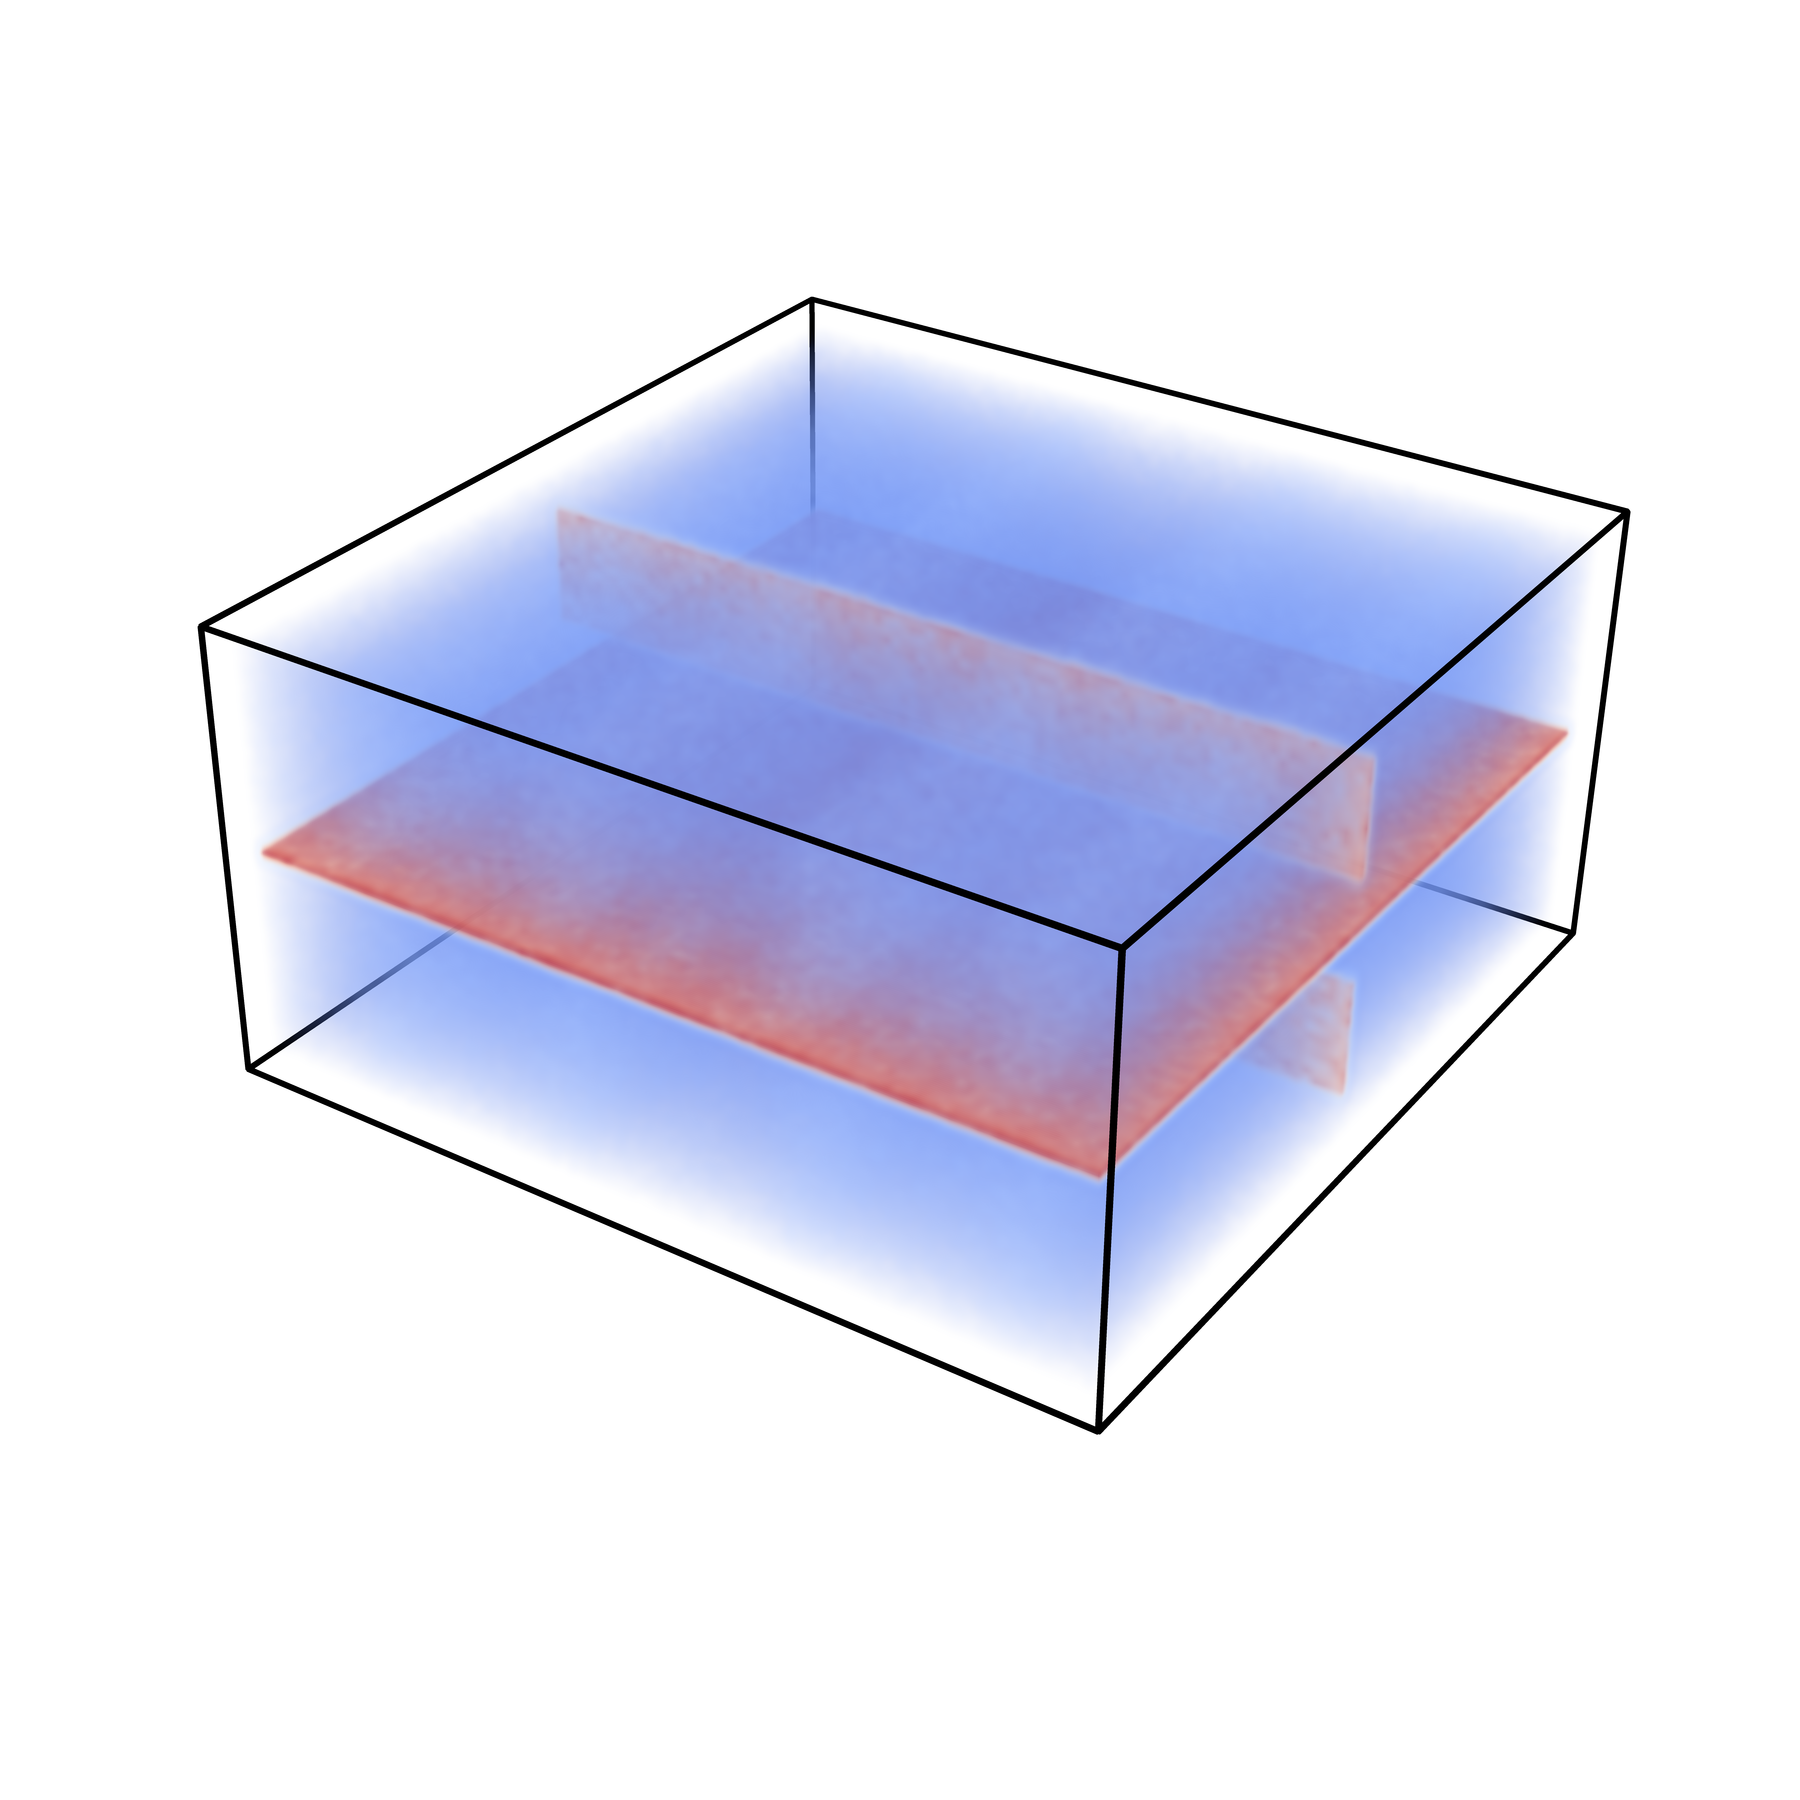
\includegraphics[trim=0 350 0 300, clip=true, width=\textwidth]{Images/shiftXeigen.png}
        \caption{Eigendecomposition}
        \label{fig:shiftXeigen}
    \end{subfigure}
    \begin{subfigure}[b]{0.49\textwidth}
        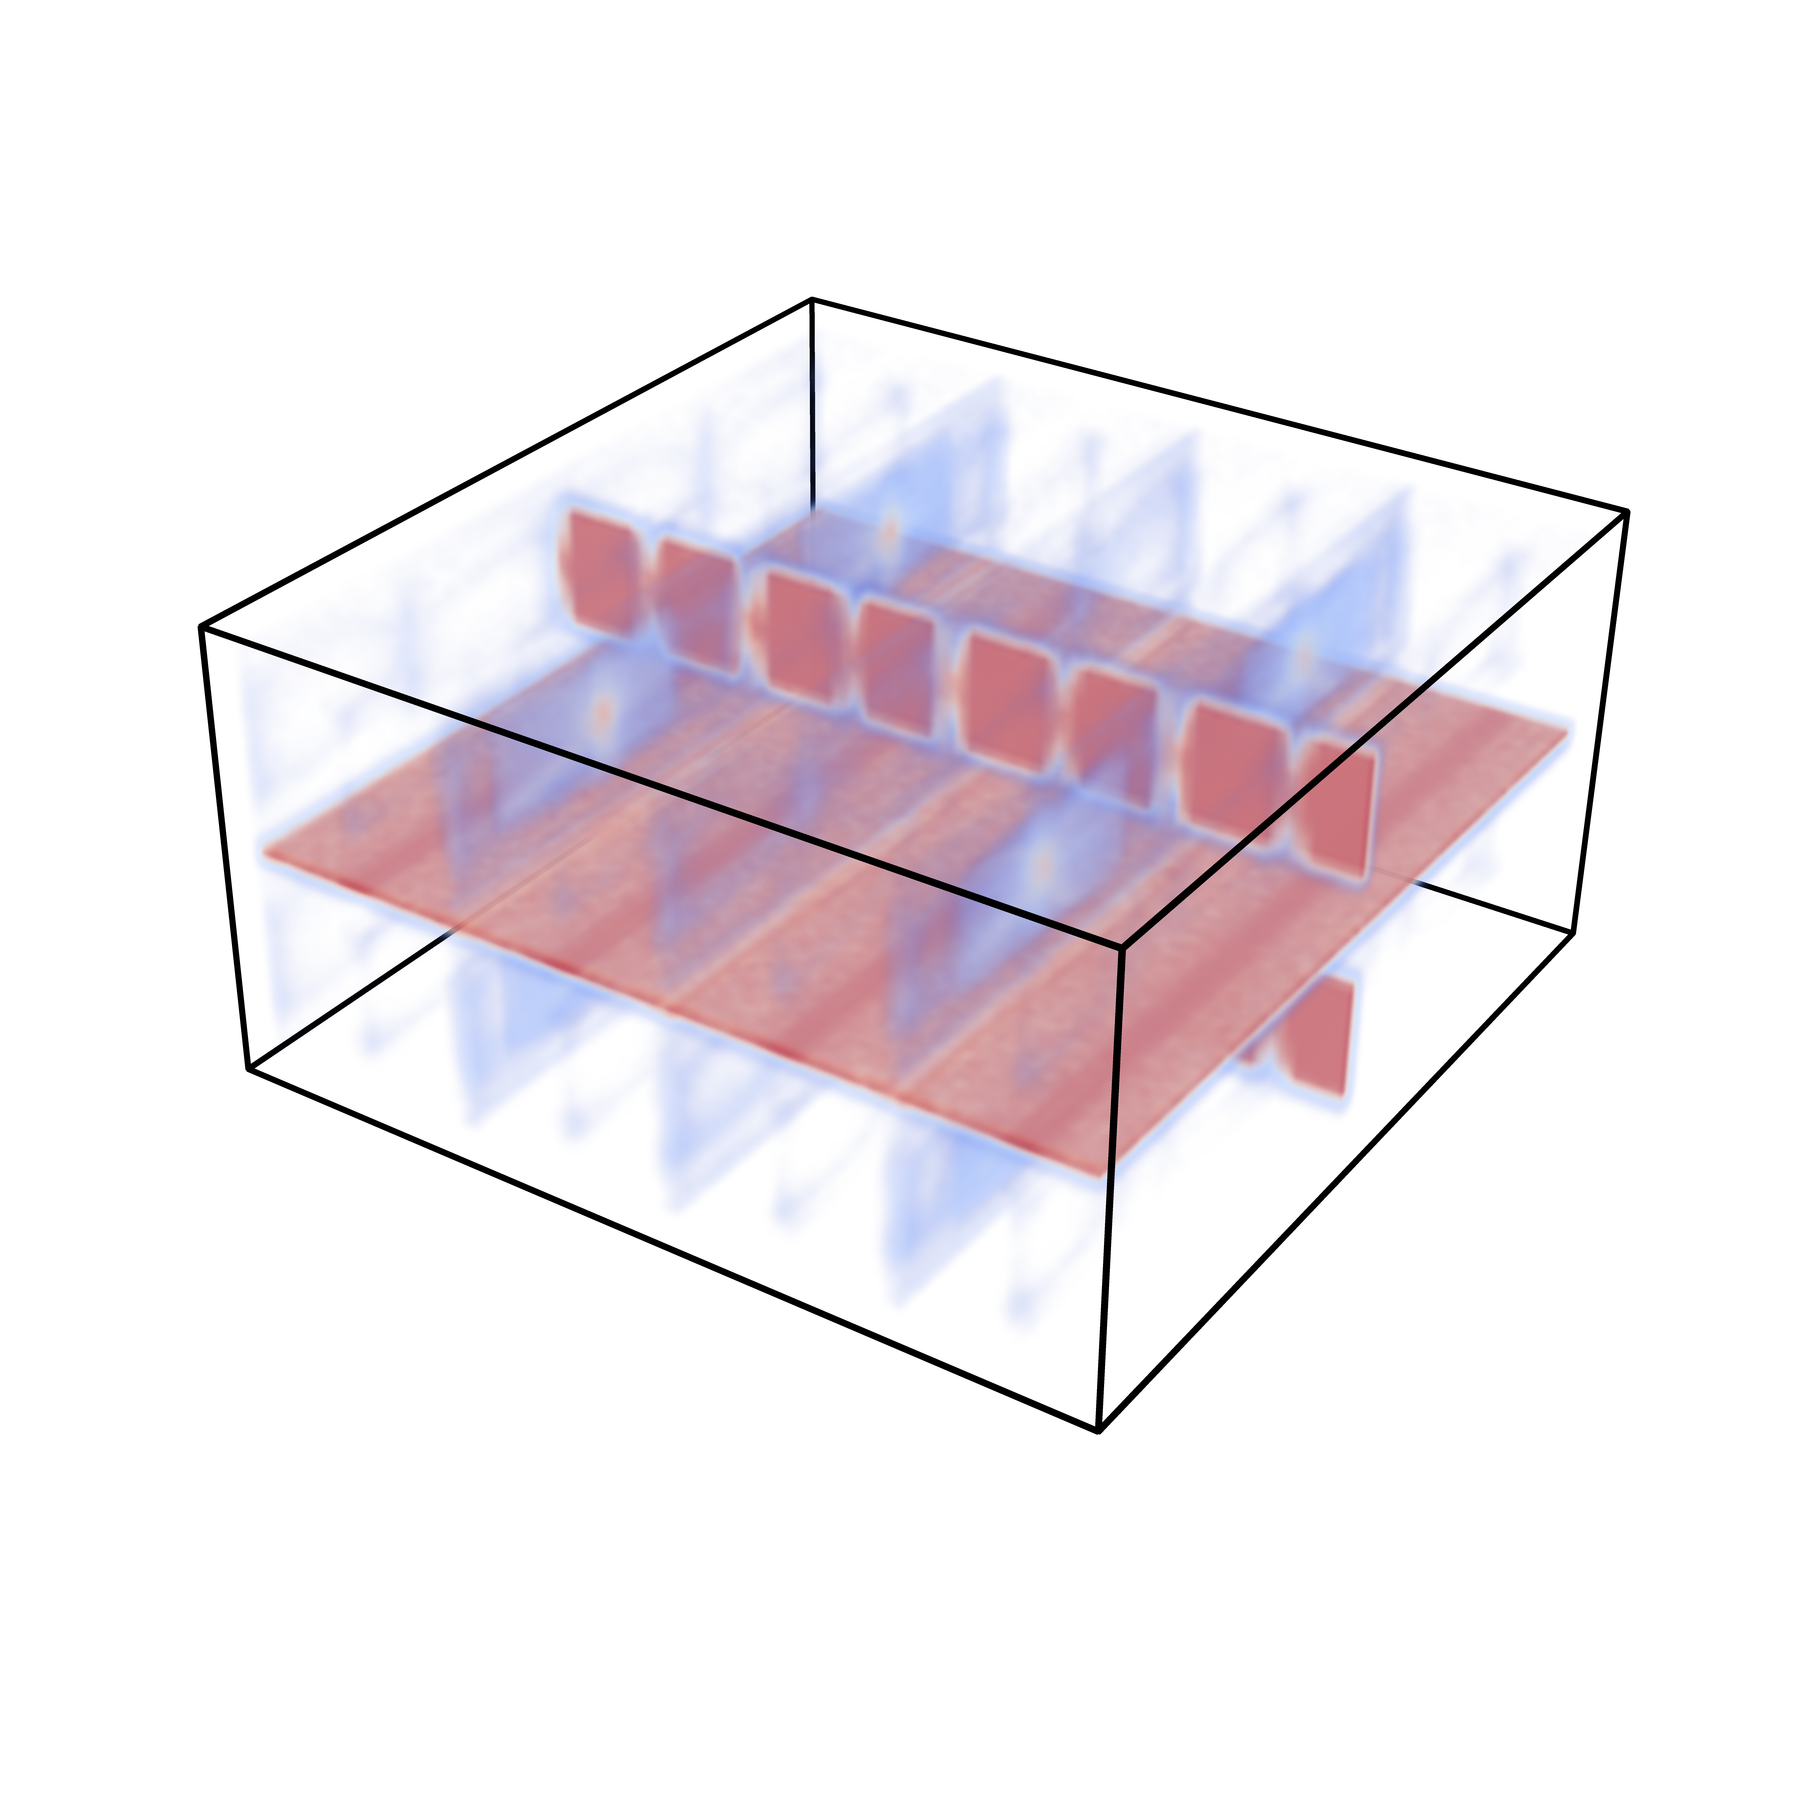
\includegraphics[trim=0 350 0 300, clip=true, width=\textwidth]{Images/shiftXcholesky.png}
        \caption{Cholesky}
        \label{fig:shiftXcholesky}
    \end{subfigure}
    \caption{Comparison of the two matrix decompositions for a set
    of fields shifted equally along the $x$ dimension. The 
    Eigendecomposition gives a smooth estimate of the ridge surface,
    according to the distribution of the ridges in the members.
    Cholesky exhibits lower probabilities at points where the
    ridge should be very certain, due to interferences.}
    \label{fig:decomps}
\end{figure}
\indent To understand what happened here, we will again take a look at
samples drawn from the distribution of Figure~\ref{fig:sampComp}.
Figure~\ref{fig:MDsampComp} shows the gradients of two samples from
either decomposition with their respective unscaled eigenvectors at the
base. Even though the Eigendecomposition in Figure~\ref{fig:sampleEig}
breaks the parallelity of the original field, the gradients still point
in the same general direction and the eigenvectors are consistently
oriented. The gradients of Cholesky on the other hand have no
directional correlation at all. The direction of the vectors is
arbitrary along the distribution and therefore their eigenvectors
have inconsistent orienting as well. The Eigendecomposition seems
to keep the correlation of elements of individual members, whereas
Cholesky mingles the members in one sample. For the calculation of
a ridge feature which depends on precision, this is an issue.\\
\begin{figure}
    \begin{subfigure}[b]{0.49\textwidth}
        \includegraphics[trim=0 350 0 100, clip=true, width=\textwidth]{Images/sampleEig.png}
        \caption{Eigendecomposition}
        \label{fig:sampleEig}
    \end{subfigure}
    \centering
    \begin{subfigure}[b]{0.49\textwidth}
        \includegraphics[trim=0 350 0 100, clip=true, width=\textwidth]{Images/sampleChol.png}
        \caption{Cholesky}
        \label{fig:sampleChol}
    \end{subfigure}
    \caption{Gradients of samples from the distribution of the rotated
    field for $f(x,y)=x^2$. The samples from the Eigendecomposition
    keep the structure of the original fields, whereas the Cholesky
    decomposition mixes the distributions in one sample.}
    \label{fig:MDsampComp}
\end{figure}
\indent The differences are the consequence of the immanent nature of the
decompositions. The Eigendecomposition of the covariance matrix
equals to the Principal Component Analysis and therefore the scaled
eigenvectors equal to the uncertainty of $\Sigma$ along
the direction of the eigenvector. If we now multiply a standard normal
distributed vector $N$ with $A = E\Lambda$, every $i$-th component of
$N$ is multiplied with a component of the $i$-th column of $A$, and thus
the $i$-th eigenvector. This leads to a constant scaling of elements
along the direction of an eigenvectors. Cholesky produces a lower
triangular matrix for $A=LD^{\frac{1}{2}}$, thus the columns have
increasing influence on the distribution of the sample with increasing
$i$, but the first element of the sample vector is only determined by
the scaling of $a_{11}$ with the random number at $N_1$. An interesting
implementation detail is, that the algorithm calculating the eigenvalues
for our large covariance matrices uses the power iteration method, that
estimates the largest absolute eigenvalue $\lambda$ in $\mathcal{O}
(N^2)$. Then the matrix is reduced by $A-\lambda I$ and power iteration
is applied again. This process can be repeated until all eigenvalues are
found. Analytic results are too computationally intensive for matrices
of size $80 \times 80$ or $24 \times 24$. Due to this algorithm, the
first column of our eigenvectormatrix always corresponds to the largest
eigenvalue, and therefore the axis with the greatest variance of the
set. Comparing this to the Cholesky decomposition, we could say that the
samples from Cholesky are mainly influenced by one axis of variance of
the data set, and decreasingly influenced by the latter variances,
resulting in more random samples.\\
\indent Ond\v{r}ej Straka \etal{\cite{MD}} studied the different matrix
decompositions in the context of Unscented Kalman Filters, but their
results are applicable for our case as well. They drew three conclusions
after their analysis of the decompositions: If the variable we want to
sample contains no correlated elements, the samples for both
decompositions are equally good and therefore the Cholesky decomposition
might be prefered because of its faster computation time. If the
variable contains correlated elements, the choice may significantly
affect the quality of the sample and, if the elements exhibit strong
correlation, numerical stability becomes an issue as well, especially
for Cholesky, as the covariance matrix with strong correlation becomes
nearly singular. Considering, that we usually apply the uncertain ridge
extraction to data sets obtained from simulations, we will have strong
correlation of the members of the data set for the most parts of the
field. The difference of the decompositions is particularly visible when
comparing the results obtained from the ridge extraction using Marching
Cubes (Figure~\ref{fig:MCcomp}). Cholesky produces the same structure as
in Figure~\ref{fig:shiftXcholesky}, but with more certainty. This is a
misleading representation of the underlying uncertainty. The results
obtained from the Eigendecomposition (Figure~\ref{fig:MCeigen}) on the
other hand can almost be considered better than the ones with our new
criterion, as the high probabilities are notably thinner distributed,
just like the certain ridge would be. We will compare the two approaches
in the next section.\\
\indent Concluding from all of this, the Eigendecomposition delivers
better results in most cases. Only if we have strong uncertainty in the
data, the Cholesky decomposition may give us better results. We took the
set from Figure~\ref{fig:MCridges} and extended it with members having
greater variance along either axis. The results of the two
decompositions can be seen in Figure~\ref{fig:HUCcomp}. The
Eigendecomposition only deliveres weak probabilities for a ridge
structure, hardly distinguishable from the surrounding noise. Here
Cholesky gives us higher probabilities for nodes close to the mean of
the ridges and, because of our criterion, not much clutter. Due to the
high variance of the data set, the members seem to lose their
correlation. The downside is, that this case is not the usual thing for
real world data, where we try to extract ridge structures from similar
scalar fields. 
\begin{figure}[]
    \begin{subfigure}[b]{0.49\textwidth}
        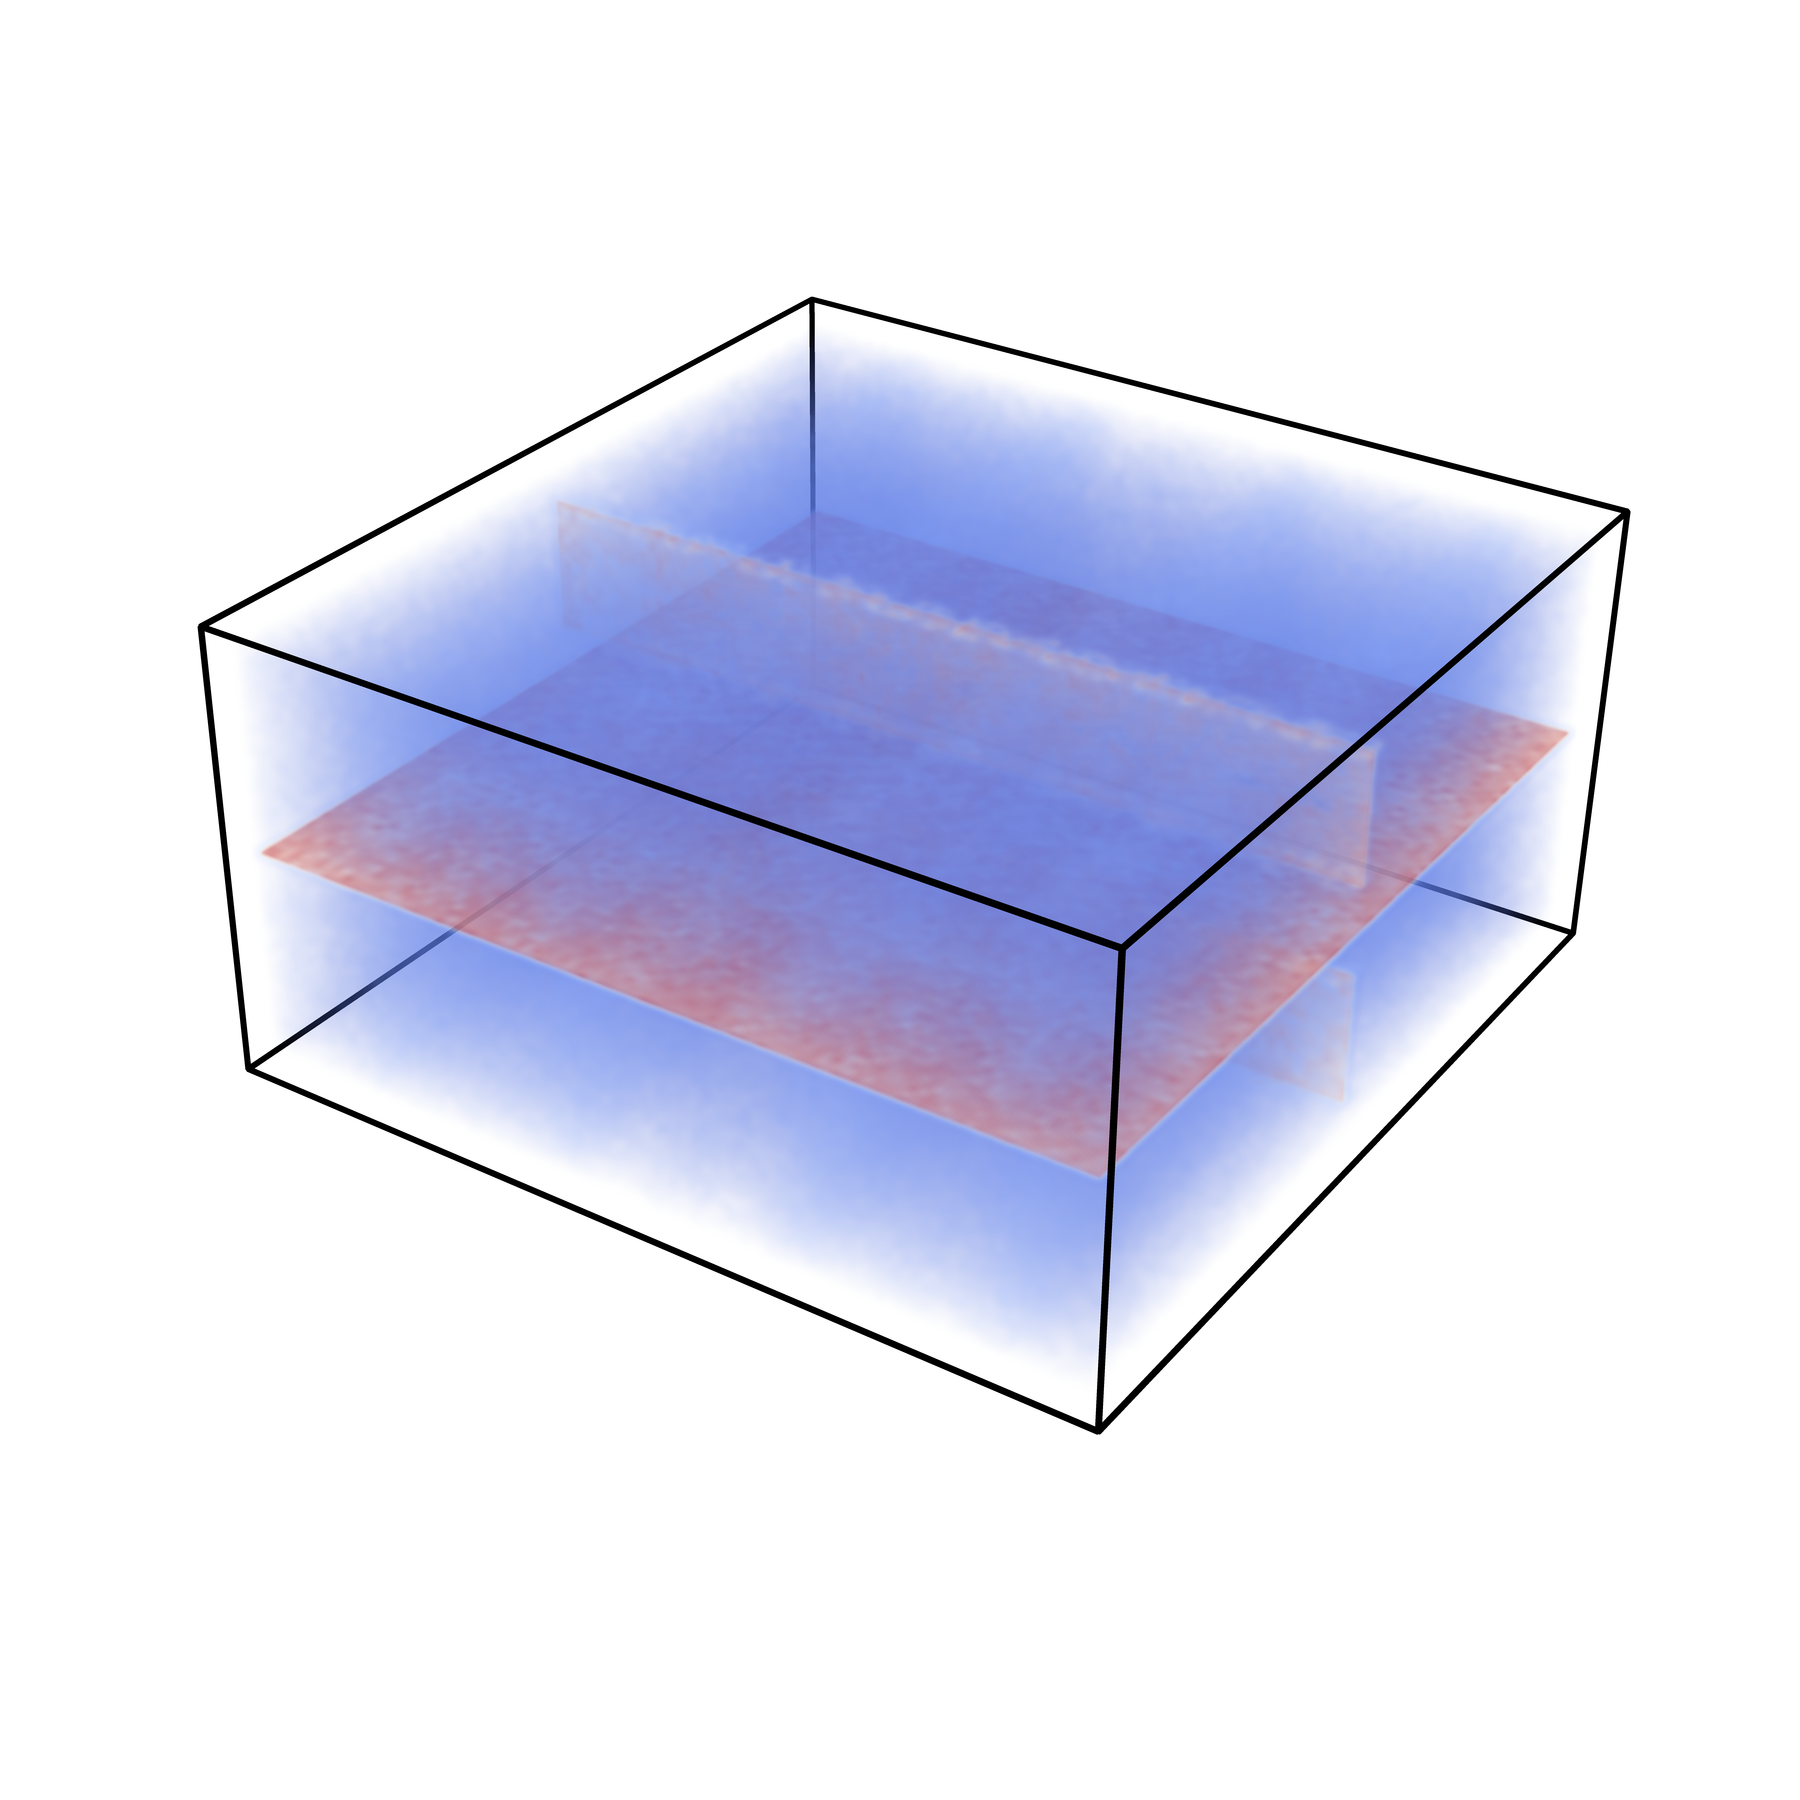
\includegraphics[trim=0 350 0 300, clip=true, width=\textwidth]{Images/shiftXold.png}
        \caption{Eigendecomposition}
        \label{fig:MCeigen}
    \end{subfigure}
    \begin{subfigure}[b]{0.49\textwidth}
        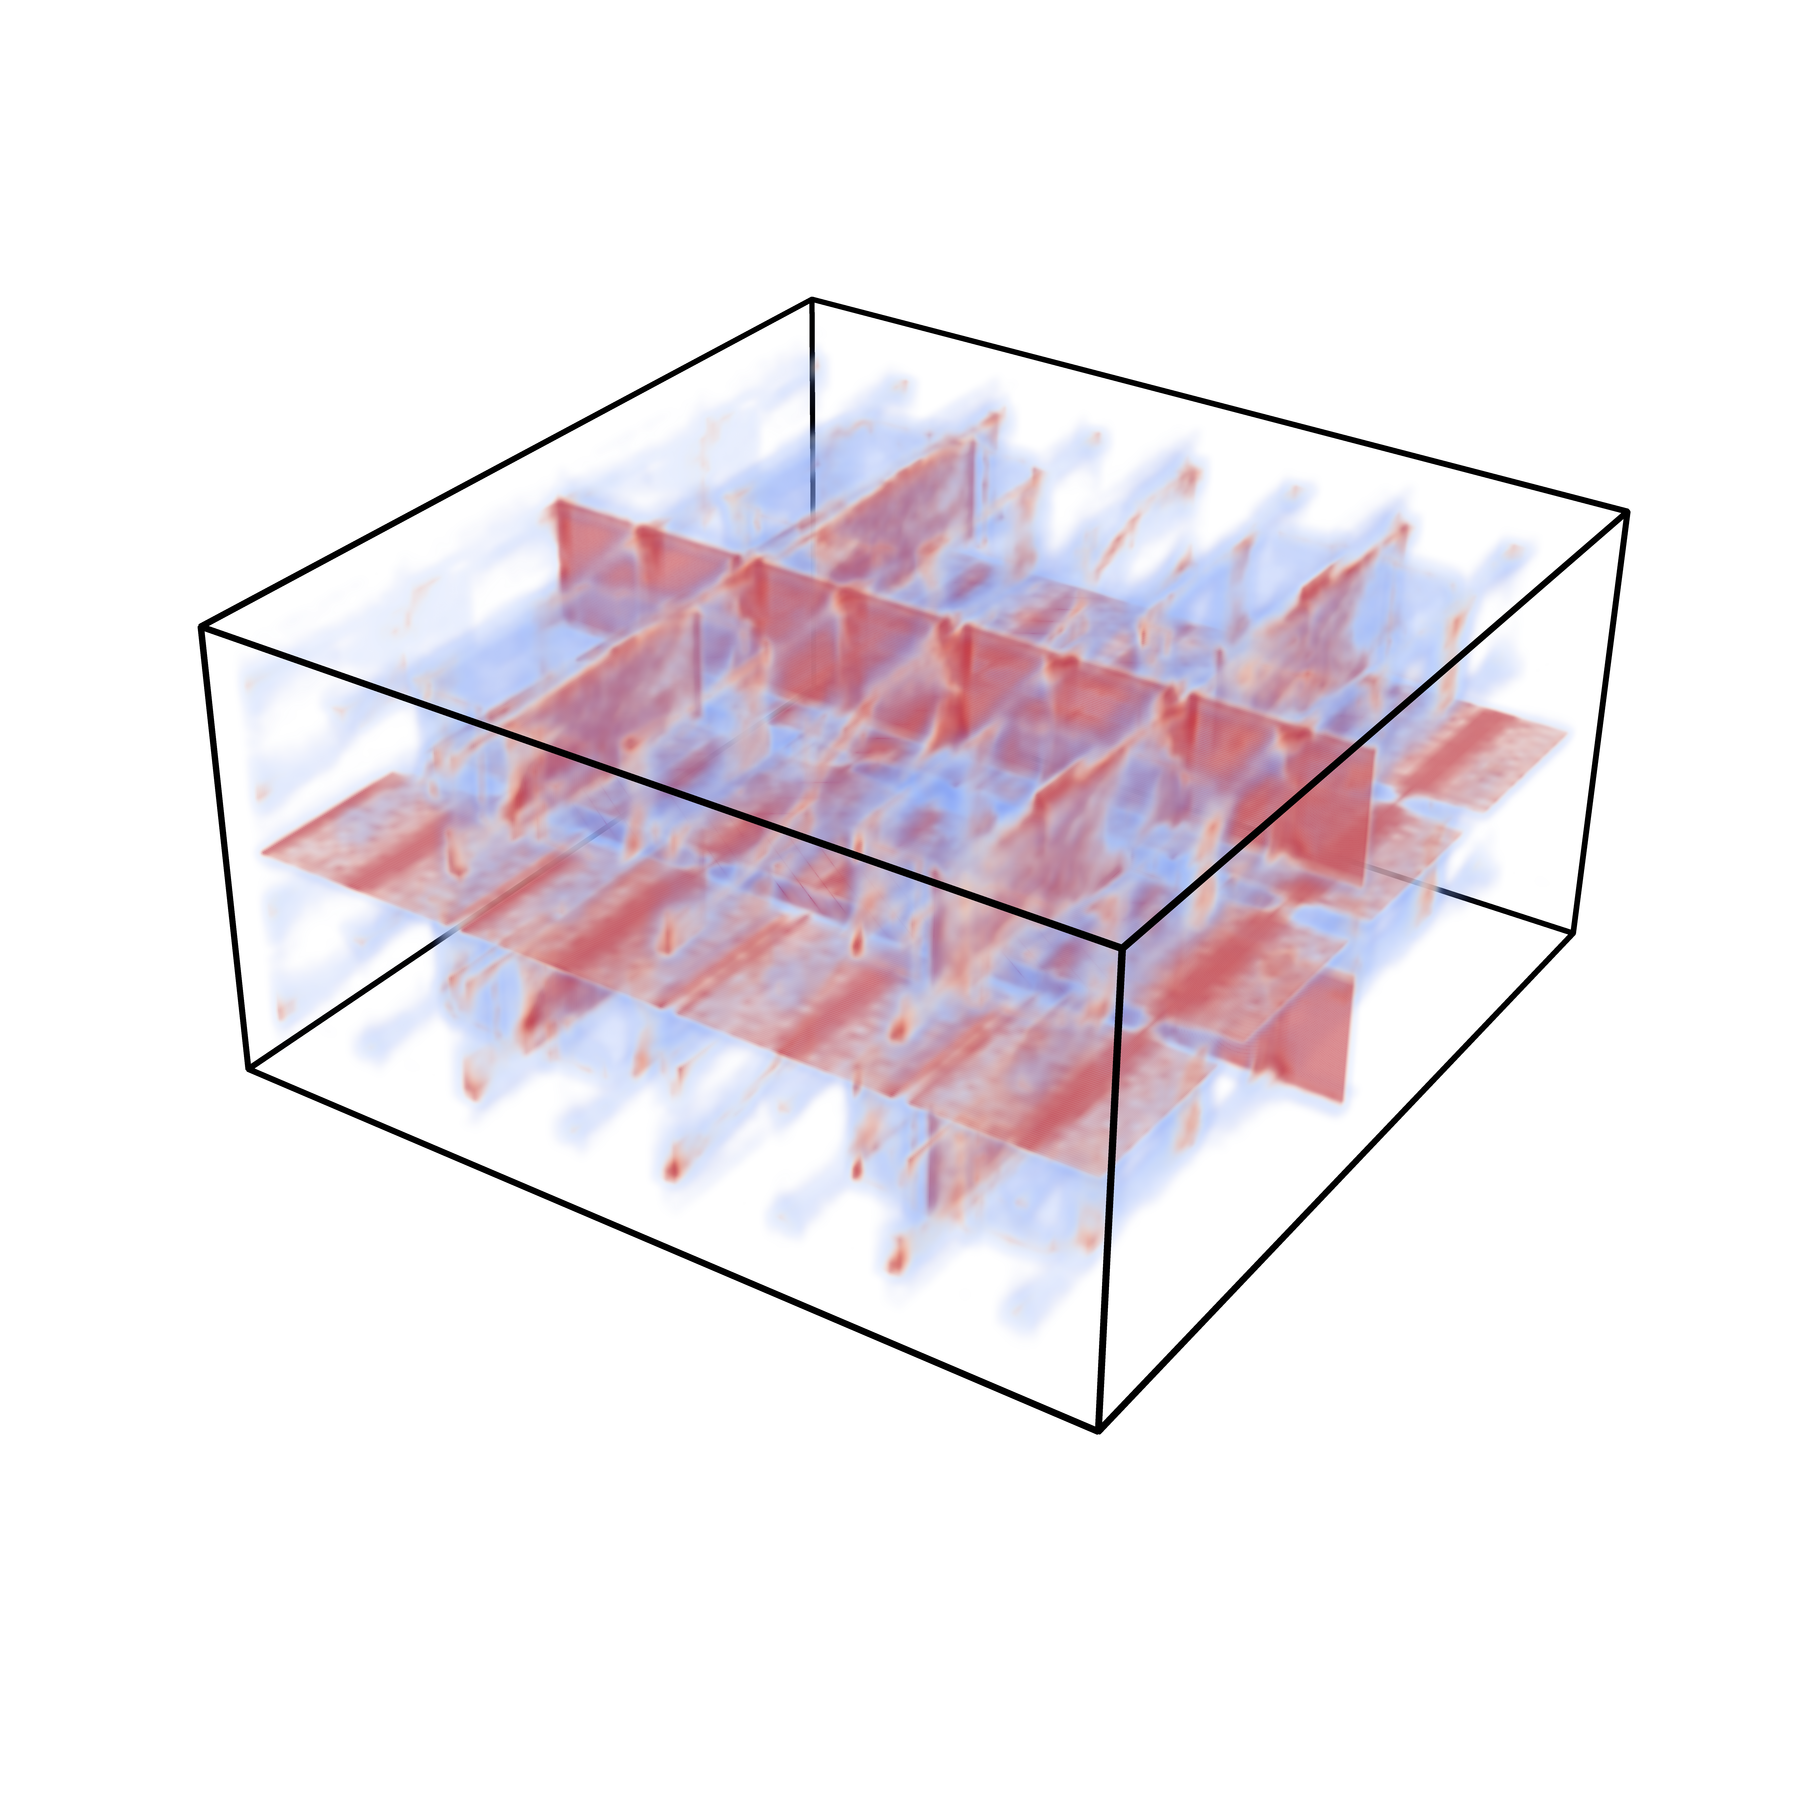
\includegraphics[trim=0 350 0 300, clip=true, width=\textwidth]{Images/shiftXoldchol.png}
        \caption{Cholesky}
        \label{fig:MCchol}
    \end{subfigure}
    \caption{Comparison of matrix decompositions for the uncertain
    ridge extraction using the Uncertain Marching Cubes algorithm. Here, the
    differences are very obvious, as UMC is strongly dependent on the relation
    of the vectors.}
    \label{fig:MCcomp}
\end{figure}
\begin{figure}
    \begin{subfigure}[b]{0.49\textwidth}
        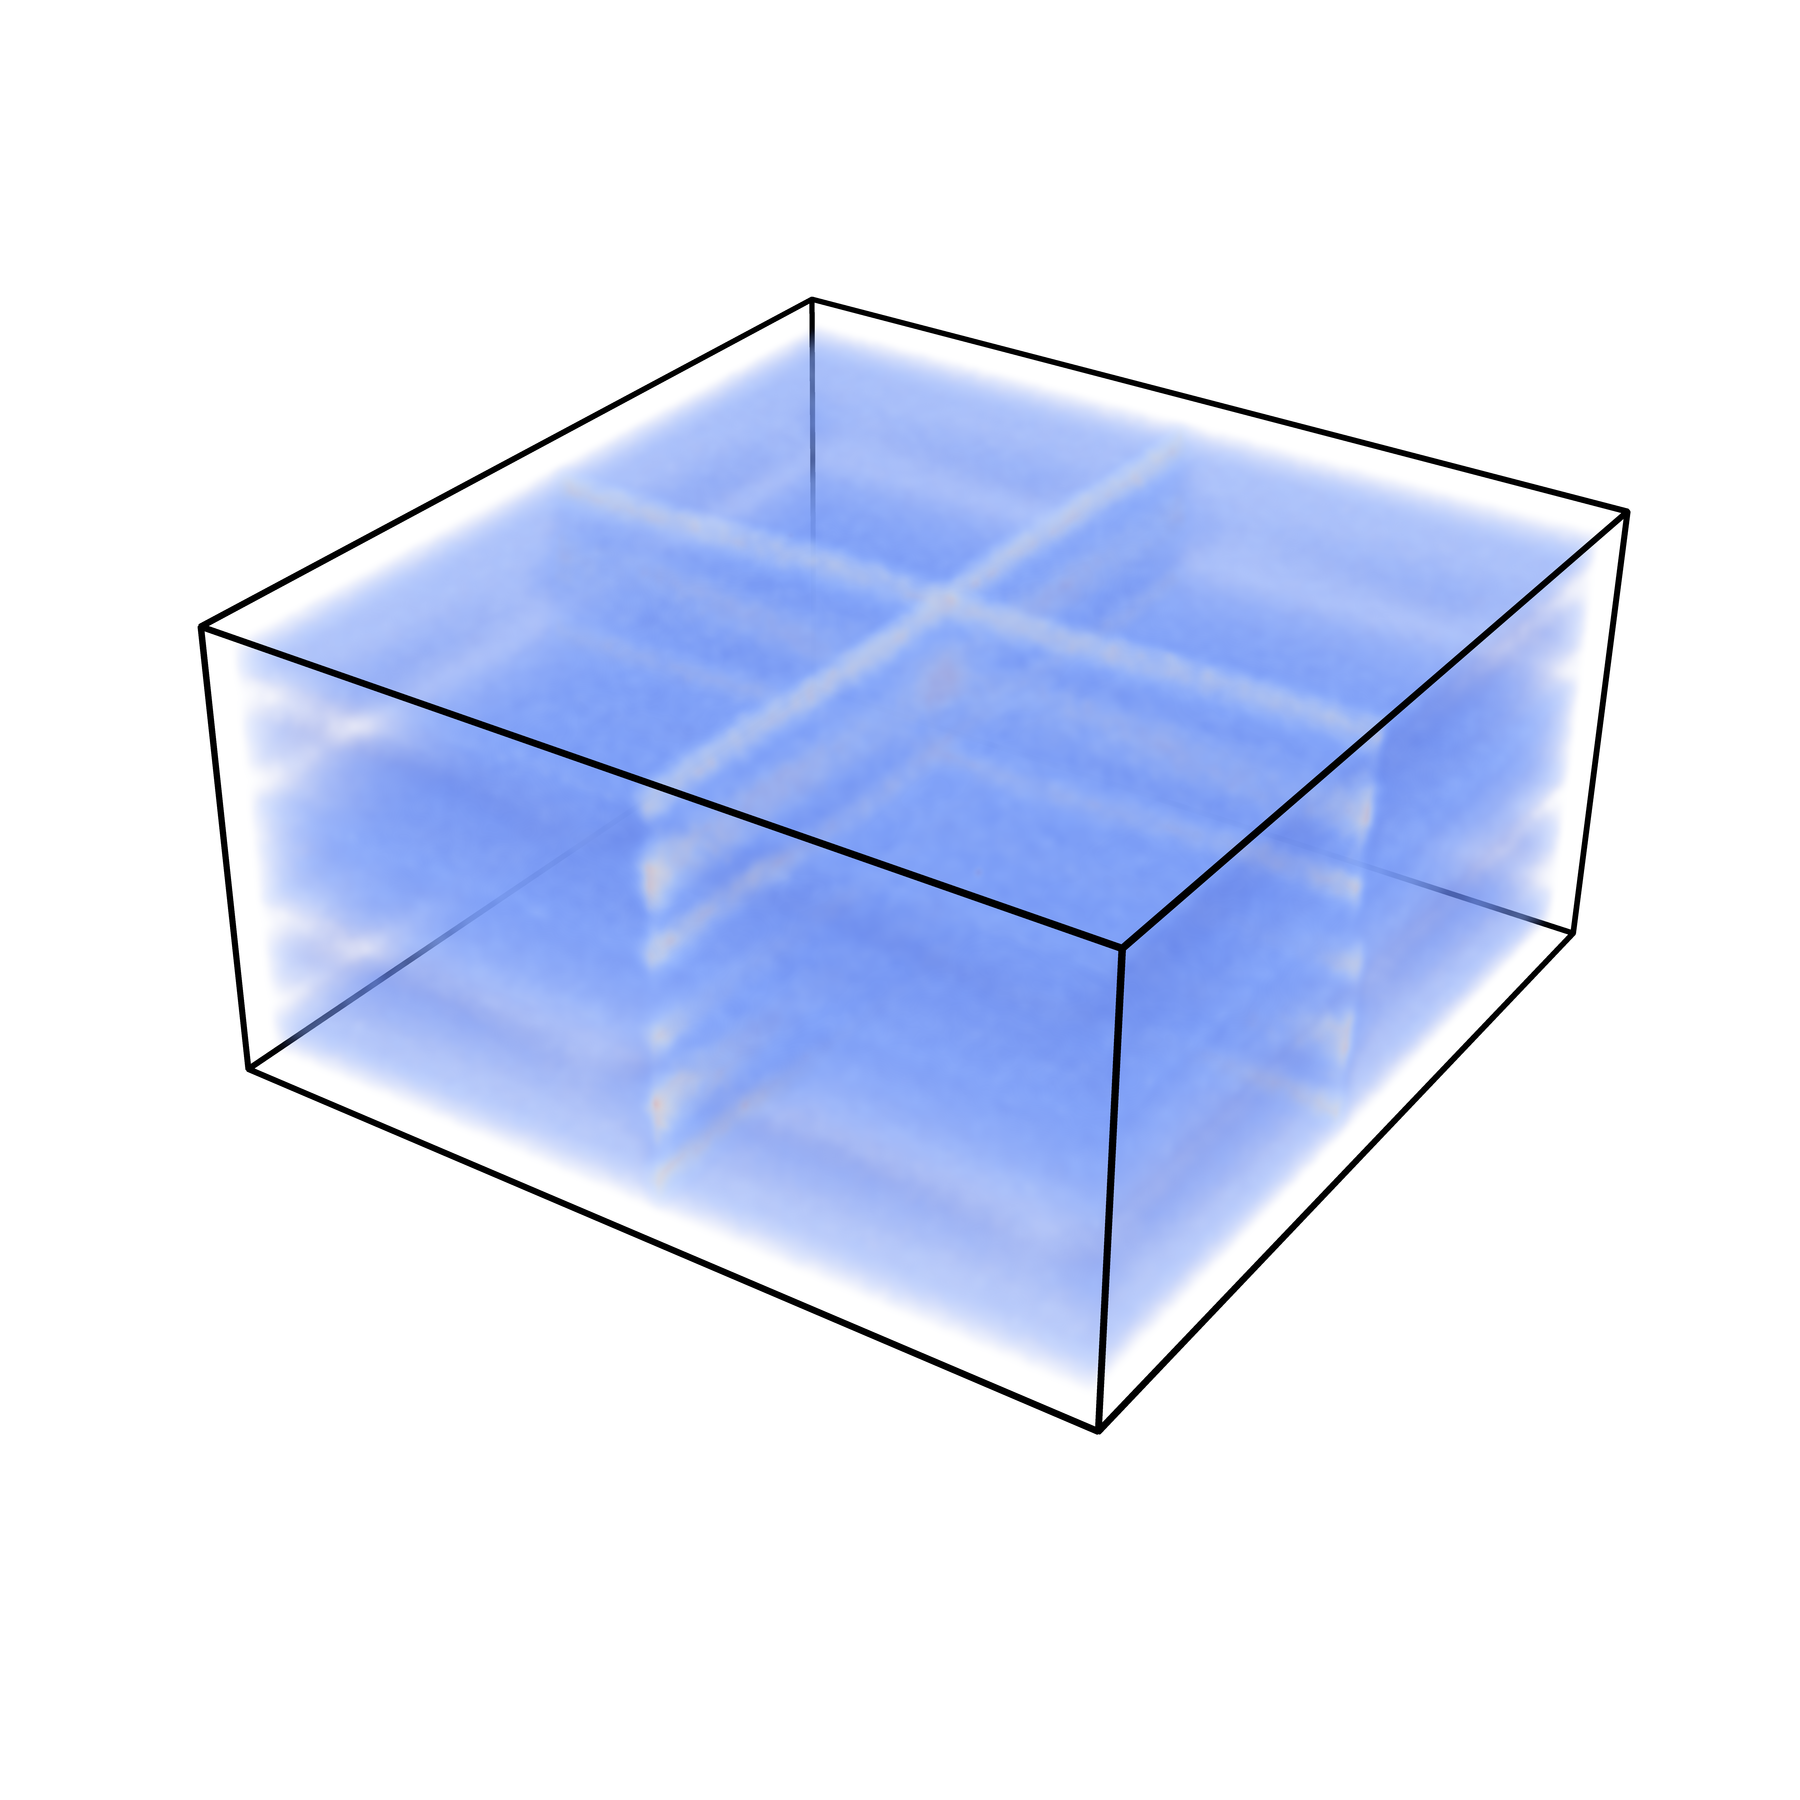
\includegraphics[trim=0 350 0 300, clip=true, width=\textwidth]{Images/highuncEigen.png}
        \caption{Eigendecomposition}
        \label{fig:HUCeigen}
    \end{subfigure}
    \begin{subfigure}[b]{0.49\textwidth}
        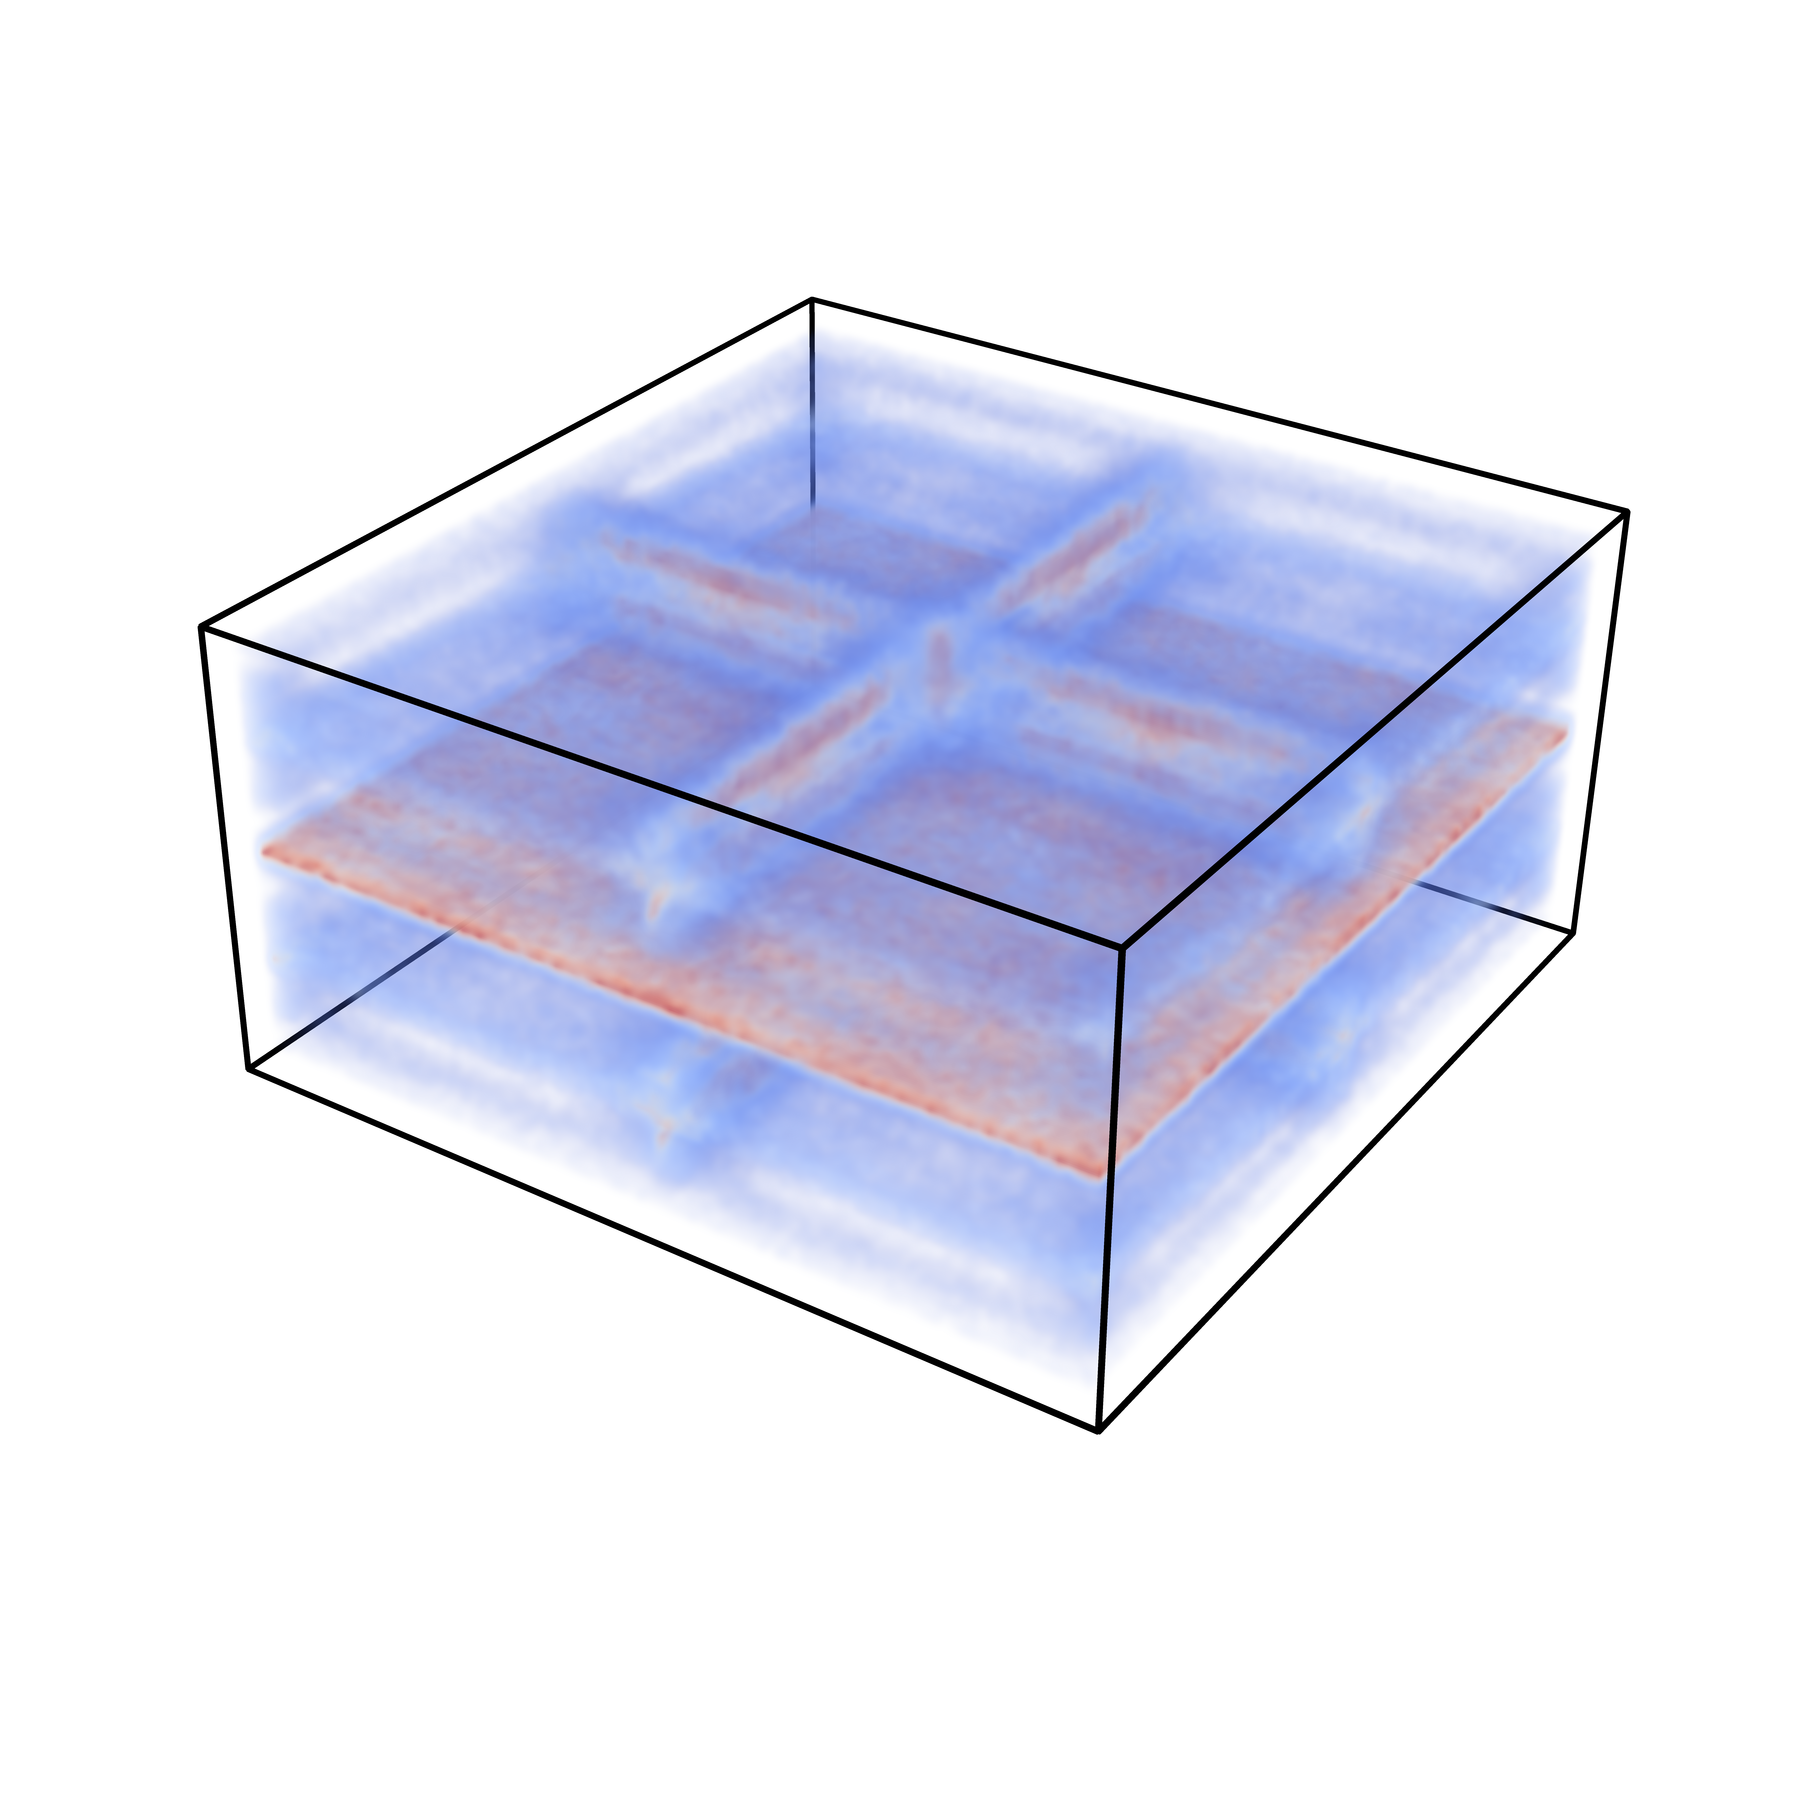
\includegraphics[trim=0 350 0 300, clip=true, width=\textwidth]{Images/highuncChol.png}
        \caption{Cholesky}
        \label{fig:HUCchol}
    \end{subfigure}
    \caption{Comparison of the matrix decompositions for a set with high
    variance in every dimension. The Eigendecomposition exhibits a ridge
    structure appearing roughly around the mean, hardly distinguishable
    from the noise surrounding it. Cholesky delivers a more certain
    structure, with parts missing from the cross like ridges on top and
    bottom, due to the up and downward distortion of the members, but
    still exhibit low probabilities.}
    \label{fig:HUCcomp}
\end{figure}

%%%%%%%%%%%%%%%%%%%%%%%%%%%%%%%%%%%%%%%%%%%%%%%%%%%%%%%%%%%%%%%%%%%%%%%%
\section{Comparison of Extraction Methods}\label{sec:evalExtr}
%%%%%%%%%%%%%%%%%%%%%%%%%%%%%%%%%%%%%%%%%%%%%%%%%%%%%%%%%%%%%%%%%%%%%%%%

After the differences of the decompositions are explained in detail, we
can proceed to evaluate the different approaches for the ridge
extraction. At first we will compare the new criterion to the extraction
with Uncertain Marching Cubes and talk about the advantages and
disadvantages. Later we will have some results for the extraction of
ridge lines in 3D.

%%%%%%%%%%%%%%%%%%%%%%%%%%%%%%%%%%%%%%%%%%%%%%%%%%%%%%%%%%%%%%%%%%%%%%%%
\subsubsection{Ridges of Co-Dimension One}\label{sec:evalMeth}
%%%%%%%%%%%%%%%%%%%%%%%%%%%%%%%%%%%%%%%%%%%%%%%%%%%%%%%%%%%%%%%%%%%%%%%%

\begin{figure}
    \begin{subfigure}{0.49\textwidth}
        \includegraphics[trim=0 450 0 450, clip=true, width=\textwidth]{Images/oldSide.png}
        \caption{Uncertain Marching Cubes}
        \label{fig:UMCside}
    \end{subfigure}
    \begin{subfigure}{0.49\textwidth}
        \includegraphics[trim=0 450 0 450, clip=true, width=\textwidth]{Images/newSide.png}
        \caption{Ridge Estimation}
        \label{fig:REside}
    \end{subfigure}
    \caption{Side view of the two extraction methods on a data set with
    no variance. \subref{fig:UMCside} UMC is creating a ridge surface
    with $100\%$ confidence for the thickness of one cell, surrounded by
    another layer of lower probability due to the tolerance $t=0.1$ for
    the dot product. \subref{fig:REside} Ridge Estimation with the
    average cell distance as $d$, offers a high confidence for 2 to 3
    layers of cells and still has another layer with lower probability
    padding it. The color difference of the upper and lower surfaces is
    due to the volume visualization of multiple high value cells in a
    row in \subref{fig:REside}.}
    \label{fig:ridgeSide}
\end{figure}

When comparing Uncertain Marching Cubes (UMC) to Ridge Estimation (RE),
the first apparent difference is the wider detection area around a ridge
for RE, as visible in Figure~\ref{fig:ridgeSide}. The areas with very
high probability in the center of the ridges are about 2 to 3 cells
thick. This is due to the estimation distance $d$, being the average
distance of two nodes in every dimension for this example. For gradients
close to a ridge, which are already almost parallel to the ridge,
Equation \ref{eq:criterion} is easily fulfilled. UMC on the other hand
deliveres full confidence only for one layer of cells. Due to the
tolerance $t=0.1$, adjacent cells get highlighted as well. This brings
us to the core difference. While the conventional approach would deliver
very certain results, Ridge Estimation gives a probability for how much
the cell was how close to a ridge over the individual members of the
ensemble.\\
\indent Our uncertain fields used in Section~\ref{sec:ridgeextract}
are generated by shifting the whole domain, yielding very little
accordance. Therefore one could argue, that the volatile regions of the
surface are indeed uncertain and therefore the holes of UMC have their
legitimacy. Real world data from simulations for example would have high
probabilities, where all the members of an ensemble have ridges and less
confident parts, where the distribution differs. Ridge Estimation would
give these locations higher probabilities, as long as the overall
structure of the ridge is similar over the members. Therefore RE can be
used to get a common shape, shared by the members at any location. The
thickness of the ridge can be adjusted with the $d$ parameter,
eventually delivering better results, but further investigation is
needed for the optimal value. RE still deliveres good results for data
sets with more congruence, but the additional detections have to be
understood to interpret the volume. If precise results for a set with a
lot of similarities are needed, UMC might be preferred.

%%%%%%%%%%%%%%%%%%%%%%%%%%%%%%%%%%%%%%%%%%%%%%%%%%%%%%%%%%%%%%%%%%%%%%%%
\subsubsection{Ridge Lines in 3D}\label{sec:evalRL3D}
%%%%%%%%%%%%%%%%%%%%%%%%%%%%%%%%%%%%%%%%%%%%%%%%%%%%%%%%%%%%%%%%%%%%%%%%

As mentioned before, we can also extract ridge lines from our uncertain
scalar fields. As the Parallel Vectors Operator is a quite precise
method, it suffers from the same problems as Uncertain Marching Cubes.
Therefore little uncertainty can already yield incomplite ridge
detections, if the data is distributed in a certain way.\\
\indent Figure~\ref{fig:doublegyre} shows the extracted ridge lines from
a simualated time-dependent double gyre field with varying parameters.
The parameters determine the amplitude of the flow and its position. The
members got slightly changed, resulting in fields with a main ridge in
the middle moving from side to side. Weaker ridge lines are in the
corners of the domain. We applied a filter for $\lambda_2$, requiring
the eigenvalue to be smaller than $0.7$ to isolate the main ridge, 
resulting in Figure~\ref{fig:dgfiltered}-

\begin{figure}
    \begin{subfigure}{0.33\textwidth}
        \includegraphics[trim=200 0 200 0, clip=true, width=\textwidth]{Images/dgyre.png}
        \caption{Double gyre}
        \label{fig:dgfield}
    \end{subfigure}
    \begin{subfigure}{0.33\textwidth}
        \includegraphics[trim=200 0 200 0, clip=true, width=\textwidth]{Images/RL3D.png}
        \caption{Raw lines}
        \label{fig:dgrawlines}
    \end{subfigure}
    \begin{subfigure}{0.33\textwidth}
        \includegraphics[trim=200 0 200 0, clip=true, width=\textwidth]{Images/RL3Dfilt.png}
        \caption{Filtered for $\lambda_2 < -0.7$}
        \label{fig:dgfiltered}
    \end{subfigure}
    \caption{Uncertain ridge line calculation for double gyre domain,
    modeling change of flow over time. \subref{fig:dgfield} Volume
    visualization of the domain from which the lines will be extracted.
    Over time, the position of the main flow moves from left to right
    and back, indicated by the lighter areas. The data set consists of
    multiple simulations of the domain with slightly adjusted parameters.
    \subref{fig:dgrawlines} Raw ridge lines over the members. The ridge
    lines at the borders of the field are distorted and artifacts are
    visible on the main ridge in the middle. \subref{fig:dgfiltered}
    Ridges filtered for $\lambda_2 < -0.7$. The smaller ridges on the
    side disappeared, only leaving the main ridge. The main ridge
    shows gaps along its line.}
    \label{fig:doublegyre}
\end{figure}

%%%%%%%%%%%%%%%%%%%%%%%%%%%%%%%%%%%%%%%%%%%%%%%%%%%%%%%%%%%%%%%%%%%%%%%%
\subsubsection{Isotropy}\label{sec:iso}
%%%%%%%%%%%%%%%%%%%%%%%%%%%%%%%%%%%%%%%%%%%%%%%%%%%%%%%%%%%%%%%%%%%%%%%%

\begin{figure}
    \centering
    \includegraphics[width=0.5\textwidth]{Images/iso.png}
    \caption{Gradients (green) around a ridge point (red) in an isotropic
    domain. The minor eigenvectors (blue) are orthogonal to their
    gradients for every point, implying the existence of a ridge line.}
    \label{fig:iso}
\end{figure}

A common problem of the extraction of $k$-dimensional ridges are areas,
where the presence of a ridge feature of lower dimensionality is
stronger than the one extracted. For example a ridge point in a
2-dimensional domain with perfect isotropy. Here, the gradient falls off
equally in either direction of the ridge feature, as the point is a
maximum along every possible direction, causing the gradient to be
almost orthogonal to its minor eigenvector in the whole area. The
gradients and their eigenvectors around a perfect ridge point are
pictured in Figure~\ref{fig:iso}. The gradients all point towards the
ridge point in the middle and don't change in any other direction. The
criterion of a ridge line is fulfilled, theoretically yielding a ridge
for the whole isotropic domain. The correct representation would only be
the point in the middle.\\
\indent Both extraction methods suffer from this problem. Figure
\ref{fig:isoEx} shows the result of the two approaches for a 3-dimensional
domain, which becomes more and more isotrope. At first, the results are
flat surfaces, but with increasing isotropy, the volumes become more
narrow until we have detections all around the perfect isotropic line.
Ridge Estimation in Figure~\ref{fig:isoRE} deliveres a full volume
all around the isotropic place, whereas Uncertain Marching Cubes still
yields some structures, due to the requirement of a change of sign
of the dot products at the cell nodes. With a higher requirement
for the eigenvalue, we can filter the size of the false detections,
but it will never become the line it should be.\\
\indent For real world data, perfect isotropy is rarely the case, but
for false detection caused by this, local areas which simulate isotropy
are still possible. In the future, this could be challenged by a filter,
deciding which dimension of ridge is dominant. This can be seen from the
eigenvalues at the respective cells, as $\lambda_2$ becomes similarly
negative to $\lambda_1$ at a ridge line in 3D. This should be a
consideration for future work.

\begin{figure}[]
    \begin{subfigure}{0.49\textwidth}
        \includegraphics[trim= 0 200 0 200, clip=true, width=\textwidth]{Images/isoRE.png}
        \caption{Ridge Estimation}
        \label{fig:isoRE}
    \end{subfigure}
    \begin{subfigure}{0.49\textwidth}
        \includegraphics[trim= 0 200 0 200, clip=true, width=\textwidth]{Images/isoUMC.png}
        \caption{Uncertain Marching Cubes}
        \label{fig:isoUMC}
    \end{subfigure}
    \caption{Comparison of the two approaches for an increasingly
    isotropic domain. \subref{fig:isoRE} Full confidence for every cell
    at perfect isotropy, leading to a volume around the correct ridge
    line with Ridge Estimation. \subref{fig:isoUMC} Similar issue for
    the Uncertain Marching Cubes algorithm, delivering false surfaces
    around the line. The size of the detected area can be minimized
    by filtering for higher eigenvalues.}
    \label{fig:isoEx}
\end{figure}

%%%%%%%%%%%%%%%%%%%%%%%%%%%%%%%%%%%%%%%%%%%%%%%%%%%%%%%%%%%%%%%%%%%%%%%%
\subsubsection{Aliasing}\label{sec:alias}
%%%%%%%%%%%%%%%%%%%%%%%%%%%%%%%%%%%%%%%%%%%%%%%%%%%%%%%%%%%%%%%%%%%%%%%%

\begin{figure}
    \centering
    \includegraphics[trim= 0 250 0 250, clip=true, width=0.5\textwidth]{Images/aliasing.png}
    \caption{Aliasing of the ridge surface in a low resolution scalar
    field. The faces yield steps, while they should be a smooth, flat
    surfaces. Supersampling is only rational for a limited amount, as it
    destroys information.}
    \label{fig:alias}
\end{figure}

Due to the cell wise extraction of the features, the minimum detection
is a whole cell. If the data sets offer low resolution, this can become
an issue. Figure~\ref{fig:alias} shows the surface for a ridge lying
aslant to the axes in a domain with low resolution. The surface becomes
blocky and the exact position of the ridge is hard to determine. This is
an issue for both extraction methods. Supersampling the domain is a
limited solution for this problem, as due to the interpolation a lot of
information is lost. The values inbetween the known locations will yield
little change, further aggravating the ridge calculation. Another
solution might be the pointwise implementation of Ridge Estimation,
together with a smaller value for $d$. This would smoothen the results,
as only close nodes get highlighted, instead of close cells. Also the
computational complexity would drop considerably, as the neighborhood,
that needs to be sampled for a single point, is fundamentally smaller.
This would also help the numerical issues coming with the Decompositions
of larger matrices.